\section{Metodología}

\subsection{Arquitectura del Sistema}

Al principio, nuestro proyecto era un desorden. Pero poco a poco fuimos organizándolo en una \textbf{arquitectura en capas} (n-tier architecture) específicamente adaptada a nuestras necesidades. La arquitectura final quedó como se muestra en la Figura~\ref{fig:arquitectura_capas}.

\begin{figure}[htbp]
    \centering
    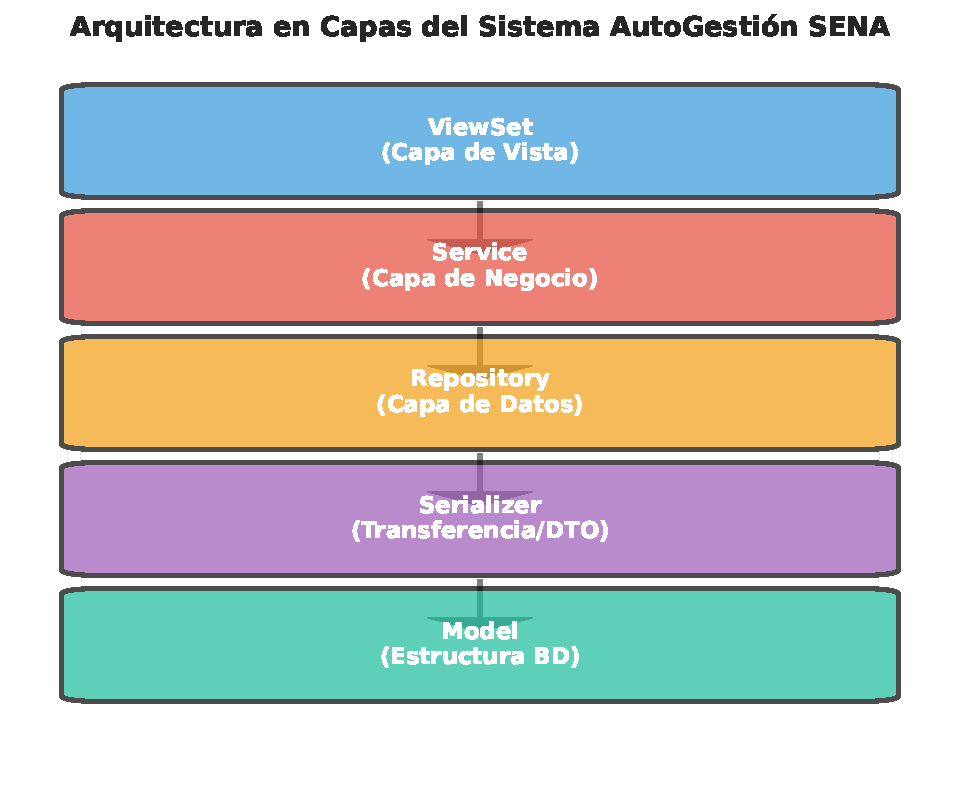
\includegraphics[width=0.48\textwidth]{graphics/arquitectura_capas.pdf}
    \caption{Arquitectura en capas del sistema AutoGestión SENA}
    \label{fig:arquitectura_capas}
\end{figure}

Esta arquitectura nos permitió:
\begin{itemize}
    \item \textbf{Separar responsabilidades}: Cada capa tiene un propósito claro
    \item \textbf{Facilitar testing}: Podemos probar cada capa por separado
    \item \textbf{Reutilizar código}: Los servicios y repositorios se pueden usar en múltiples lugares
    \item \textbf{Mantener el código limpio}: Sin mezclar lógica de diferentes niveles
\end{itemize}

\subsection{Tecnologías Utilizadas}

Para que esto funcionara, usamos tecnologías modernas y potentes:

\textbf{Backend}:
\begin{itemize}
    \item \textbf{Python 3.11}: Lenguaje principal
    \item \textbf{Django 4.2}: Framework web
    \item \textbf{Django REST Framework}: Para crear la API REST
    \item \textbf{MySQL 8.0}: Base de datos relacional
    \item \textbf{Celery}: Para tareas asíncronas (envío de correos, notificaciones)
    \item \textbf{Redis}: Como broker para Celery y caché
    \item \textbf{Docker}: Para containerización
\end{itemize}

\textbf{Frontend}:
\begin{itemize}
    \item \textbf{React 18}: Biblioteca de UI
    \item \textbf{TypeScript}: Para tipado estático
    \item \textbf{Vite}: Build tool moderno
    \item \textbf{Tailwind CSS}: Framework de estilos
    \item \textbf{Fetch API}: Para comunicación con el backend
\end{itemize}

\subsection{Patrones de Diseño Aplicados}

\subsubsection{Repository Pattern}

Este patrón nos ayudó a separar la lógica de acceso a datos de la lógica de negocio. En lugar de hacer consultas directamente en los servicios o vistas, creamos repositorios que encapsulan todas las operaciones con la base de datos.

\textbf{Ventajas que obtuvimos}:
\begin{itemize}
    \item Consultas centralizadas y optimizadas
    \item Fácil de testear con mocks
    \item Cambios en la base de datos solo afectan a los repositorios
    \item Código más limpio y legible
\end{itemize}

\subsubsection{DTO Pattern (Data Transfer Object)}

En nuestro caso, usamos \textbf{Serializers de Django REST Framework} como DTOs. Estos nos permiten:
\begin{itemize}
    \item Validar datos de entrada
    \item Transformar modelos a JSON
    \item Controlar qué campos se exponen en la API
    \item Separar la representación de datos de los modelos internos
\end{itemize}

\subsubsection{Service Layer Pattern}

Los servicios encapsulan toda la lógica de negocio. No acceden directamente a los modelos, sino que usan los repositorios.

\textbf{Ventajas}:
\begin{itemize}
    \item Lógica de negocio centralizada
    \item Fácil de testear
    \item Reutilizable en múltiples endpoints
    \item Separación clara de responsabilidades
\end{itemize}

\subsection{Buenas Prácticas Aplicadas}

\subsubsection{Clean Code}

Siguiendo los principios de Martin~\cite{martin2008clean}:
\begin{itemize}
    \item \textbf{Nombres descriptivos}: Variables y funciones con nombres claros
    \item \textbf{Funciones pequeñas}: Cada función hace una sola cosa
    \item \textbf{Comentarios útiles}: Solo donde realmente aportan valor
    \item \textbf{DRY (Don't Repeat Yourself)}: No duplicar código
\end{itemize}

\subsubsection{Principios SOLID}

Aunque suene muy ``pro'', los principios SOLID son super lógicos:
\begin{itemize}
    \item \textbf{S}ingle Responsibility: Cada clase tiene una responsabilidad
    \item \textbf{O}pen/Closed: Abierto para extensión, cerrado para modificación
    \item \textbf{L}iskov Substitution: Las clases hijas pueden sustituir a las padres
    \item \textbf{I}nterface Segregation: Interfaces específicas
    \item \textbf{D}ependency Inversion: Depender de abstracciones
\end{itemize}

\subsubsection{Validaciones}

Validamos los datos en todos los niveles posibles para evitar errores:
\begin{itemize}
    \item \textbf{Frontend}: Validación de formularios con React
    \item \textbf{Serializer}: Validación de tipos y formatos
    \item \textbf{Service}: Validación de reglas de negocio
    \item \textbf{Base de datos}: Constraints y foreign keys
\end{itemize}

\subsection{Proceso de Desarrollo}

El proyecto evolucionó en varias etapas, como se muestra en la Figura~\ref{fig:evolucion_proyecto}:

\begin{figure}[htbp]
    \centering
    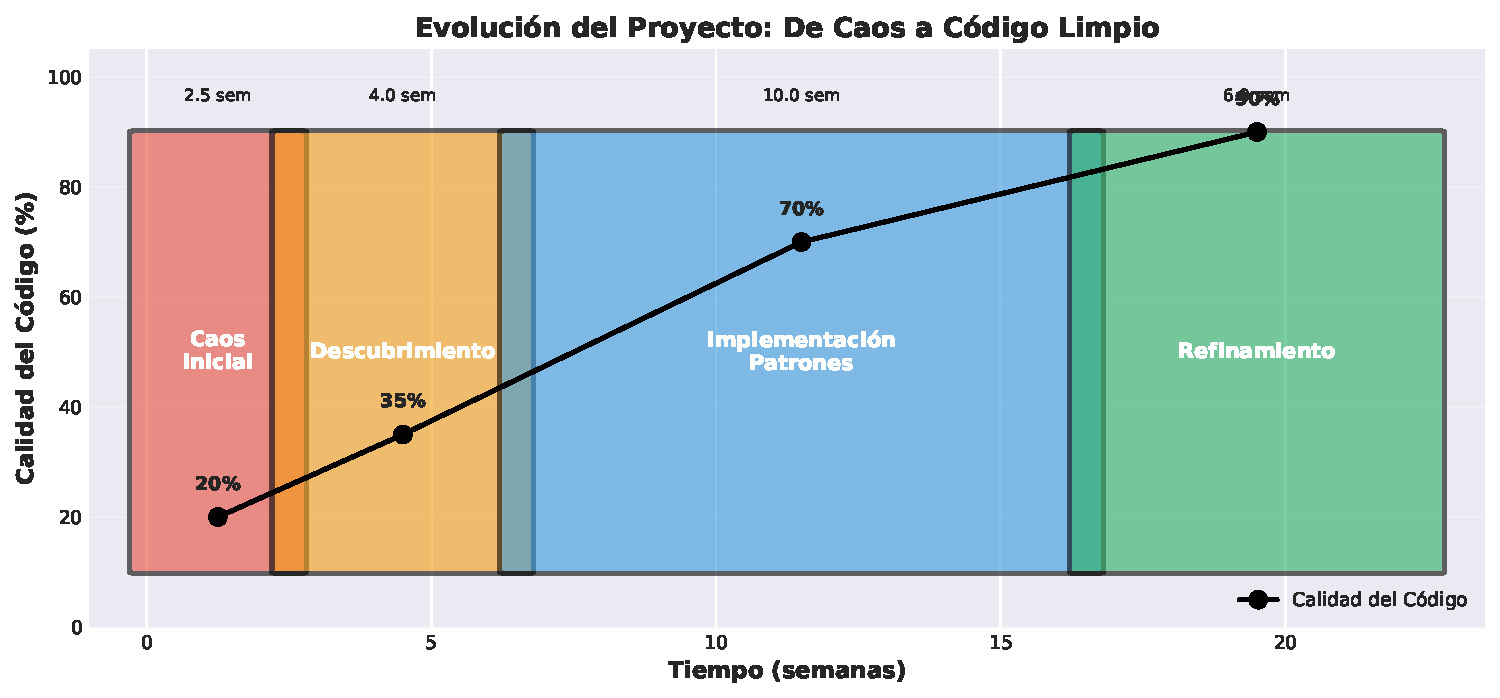
\includegraphics[width=0.48\textwidth]{graphics/evolucion_proyecto.pdf}
    \caption{Evolución del proyecto en el tiempo: de caos a código limpio}
    \label{fig:evolucion_proyecto}
\end{figure}

\begin{itemize}
    \item \textbf{Etapa 1: Caos Inicial (2-3 semanas)}: El desorden. Código mezclado y cero estructura.
    \item \textbf{Etapa 2: Descubrimiento (1 mes)}: Nos dimos cuenta de la gravedad y empezamos a investigar patrones.
    \item \textbf{Etapa 3: Implementación de Patrones (2-3 meses)}: El refactoring fuerte. Creamos las capas de Repository y Service.
    \item \textbf{Etapa 4: Refinamiento (1-2 meses)}: Optimizamos consultas, documentamos y pulimos los detalles.
\end{itemize}